\section{Postflop Strategy}
Reaching the flop means we have access to more information that enables us to conceptualize how the hand will progress. Usually, as the round progress, the number of active opponents decreases, making it easier to estimate the strength of our hand. In the next section, we will explore how PokerShark estimates the strength of its pocket.

\subsection{Hand Strength}
We need to define a metric that enables us to assess how our pocket would perform against the hands of the opponents. Numerous methods were proposed in the literature, such as Artificial Neural Networks\cite{bensson2013predicting}, Monte Carlo analysis, and enumeration \cite{billings_challenge_2002}.

Before discussing hand strength, we need to solve the problem of comparing two hands. There are three community cards on the flop, and each player has two pocket cards, which means a 5-card hand can already be constructed. So if the opponents show their cards, how can we tell which hand is the strongest?

\subsubsection{Absolute Hand Rank}
Comparing hands is not trivial, but it can be done efficiently using the absolute hand rank, which is a numerical value assigned to each possible hand that allows us to compare hand strength.
There are many implementations of the absolute hand rank, but most implementations are based on Cactus Kev's Algorithm\footnote{\url{https://suffe.cool/poker/evaluator.html}}. Although we do not want to go extensively into this topic, we will provide a high-level outline. There are $2598960$ unique possible hand combinations, but most hands are not distinct. For example, \card{H}{A}\card{D}{A}\card{C}{A}\card{S}{A}\card{H}{K} and  \card{H}{A}\card{D}{A}\card{C}{A}\card{S}{A}\card{D}{K} are unique hands but have the same rank.

If we only consider distinct hands, we have only 7462 different combinations, which is manageable.

% table of distinct hands
\begin{table}[h]
    \centering
    \begin{tabular}{|c|c|c|}
        \hline
        \textbf{Hand Value}      & \textbf{Unique}  & \textbf{Distinct} \\\hline
        Straight Flush  & 40      & 10       \\\hline
        Four of a Kind  & 624     & 156      \\\hline
        Full Houses     & 3744    & 156      \\\hline
        Flush           & 5108    & 1277     \\\hline
        Straight        & 10200   & 10       \\\hline
        Three of a Kind & 54912   & 858      \\\hline
        Two Pair        & 123552  & 858      \\\hline
        One Pair        & 1098240 & 2860     \\\hline
        High Card       & 1302540 & 1277     \\\hline
        \textbf{TOTAL}           & \textbf{2598960} & \textbf{7462}     \\\hline
    \end{tabular}
    \caption{Number of unique and distinct hands}
    \label{tab:unique}
\end{table}

These combinations are ordered into a hash table with an index representing the hand's value. Finally, an encoding function is used to create a hand mask that can be used to look up the hand's value using the hash table. This algorithm enables us to compare hands efficiently, which is a very important tool that we will utilize in estimating hand strength. We have to note here that the following methods and algorithms are heavily influenced by \cite{billings_challenge_2002},\cite{papp_dealing_1998}, and \cite{davidson_improved_2000}.


\subsection{Facing one Opponent}
when facing one opponent post-flop enumerating all his possible pockets is not computationally hard. The deck of cards has 52 cards, we have two cards, and on the flop, we get to see three of the board cards, leaving the opponent with ${47 \choose 2} = 1081$ possible combinations that a modern  CPU can enumerate through in a matter of milliseconds. The number of possible combinations only goes down as the round progress.

\begin{Algorithmus}[H]
    \caption{Hand Strength estimation against one opponent}
    \label{alg:enum}
    \begin{algorithmic}
        \Procedure{HandStrength}{$Pocket, Board$}
        %\State $Wins, Count  \gets 0$
        \State $PocketRank \gets GetAbsoluteHandRank(Pocket | Board)$
        \For {$OpponentHand \in GetPossibleHands(Pocket, Board)$}
            \State $OpponentRank \gets GetAbsoluteHandRank(OpponentHand)$
            \If {$OpponentRank > PocketRank$}
                \State $Wins \gets Wins + 1$
            \EndIf
            \If {$OpponentRank = PocketRank$}
                \State $Wins \gets Wins + 0.5$
            \EndIf
            \State $Count \gets Count + 1$
        \EndFor
        \State \Return $Wins / Count$
        \EndProcedure
    \end{algorithmic}
\end{Algorithmus}

Algorithm \ref{alg:enum} is used to deliver the win odds of our hand by iterating throw all possible opponent hands. We consider a draw as half as good as a win. Although the algorithm might seem very reasonable at first glance, it does not consider opponent preferences, which is a significant weakness because post-flop, almost all of the weak hands have already been folded. Many of the wins we are counting toward hand strength have no value in practice. Let us consider the following board: \card{C}{Q}\card{S}{Q}\card{D}{J}\card{H}{7}\card{D}{3} and the pocket \card{C}{A}\card{D}{K}. The previous algorithm will assume all opponent's hands are equally likely and will give a 0,51 win odds. If we are facing a tight opponent with a range similar to the one shown in figure \ref{fig:tight}, the actual win odds are closer to 0,12 which is a big difference.

\begin{figure}[h]
    \centering
    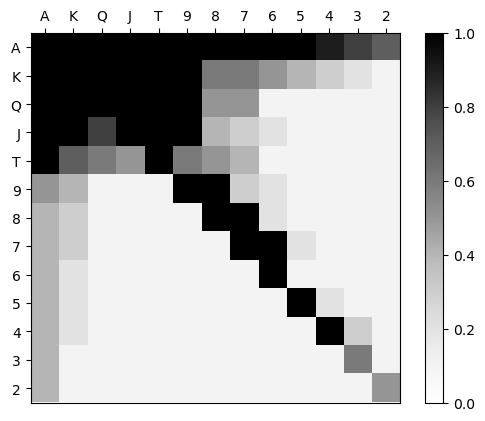
\includegraphics[width=0.5\textwidth]{tight.png}
    \caption{Tight opponent range}
    \label{fig:tight}
\end{figure}

Here is where adjustment matrices and opponent models prove valuable. We can adjust the algorithm to weigh each win/draw resulting in a much more accurate estimation.

\subsection{Hand Potential}

One very important factor that we need to take into consideration when assessing hand strength is how future board cards are going to affect our pocket. For example, our pocket is \card{H}{8}\card{H}{7} and a board of \card{H}{A}\card{H}{T}\card{S}{3} the direct hand strength of our hand is low 0,18 (assuming the opponent has no preferred range). However, any heart card will give us a flush. With a seven or eight, we can get one or two pairs. Nine and six or Jack and nine will make a straight. The hand has a significant chance to improve with two board cards remaining.
We use The \textit{HandPotential2} Algorithm from \cite{papp_dealing_1998}, which returns the probability of our hand improving PP and the probability of our hand worsening NP.